\documentclass[mathserif]{beamer}
\usetheme{Berlin} %sidebar
\usecolortheme{dolphin}
\newcommand{\bi}{\begin{itemize}\item}
\newcommand{\ei}{\end{itemize}}
\renewcommand{\vec}[1]{\mathbf{#1}}

\newcommand{\inner}[2]{\big<\vec{#1}\cdot\vec{#2}\big>}
%\include{../beamer_presentation}

\usepackage{tabularx}
\usepackage{graphicx}
\graphicspath{{figs/}}
\DeclareGraphicsExtensions{.eps}

\title[Sampling Strategies in Ordinal Regression for Surrogate Assisted Evolutionary Optimization \qquad\qquad\qquad\quad\qquad\qquad\; (ISDA 11)]{Sampling Strategies in Ordinal Regression for Surrogate Assisted Evolutionary Optimization}
\author{Helga Ingimundardottir \& Thomas Philip Runarsson}
\date{November 24th, 2011} % beskidt .. men det virker
\institute{School of Engineering and Natural Sciences, University of Iceland}

%\beamertemplatenavigationsymbolsempty % fjerner pdf-indhold

%\AtBeginSection[]{\begin{frame}<beamer>   \frametitle{Overview}    \tableofcontents[currentsection]  \end{frame} }


%%%%%%%%%%%%%%%%%%%%%%%%%%%%%%%%%%%%%%
\begin{document}
%%%%%%%%%%%%%%%%%%%%%%%%%%%%%%%%%%%%%%
\frame{\titlepage}

\frame{\frametitle{Overview}
\begin{enumerate}
 \item Introduction
 \item Ordinal Regression
 \item Sampling Methods and Improvements
 \item Experimental Study
 \item Main Conclusions
 \item Future Work
\end{enumerate}

}

\section{Introduction}\subsection{Introduction}
\frame{\frametitle{Motivation}
During evolution, different regions of space are sampled and as a consequence the surrogate ranking model may be insufficiently accurate for new regions of the search space. 
\vspace{1cm}\\
Hence if the surrogate is  not updated to reflect the original fitness function it is very probable that the ES converges a false optimum.
}
\frame{\frametitle{Goal}
\bi General goal is how to validate goodness of fit for surrogate models during search 
  \item Introducing a novel validation/updating policy 
  \item Illustrated on classical numerical optimisation problems
\ei
}
\frame{\frametitle{Previous work}
Methods previously proposed for validating surrogate models:
  \bi Validating on entire vs. subset of candidate population (Ratle, 1999), e.g. accurate ranking of potential parent individuals (Runarsson, 2004)
  \item Generation based or individual based (Jin, 2005)
\ei 
}

\section{Ordinal Regression}\subsection{Ordinal Regression}
\frame{\frametitle{Ordinal regression}
\bi Mapping of points to ranks: $ \{h(\cdot) : X \mapsto Y\}$
\bi $\vec{x}_i \succ \vec{x}_j \quad \Leftrightarrow \quad h(\vec{x}_i) > h(\vec{x}_j)$ \ei
\item Ordinal regression: obtain function $h^*$ that can for a given pair $(\vec{x}_i,y_i)$ and $(\vec{x}_j,y_j)$ distinguish between two different outcomes: $y_i > y_j$ and $y_j > y_i$. 
\item Problem of predicting the relative ordering of all possible pairs of examples
\ei
The surrogate considered may be defined by a linear function in the feature space (of dimension $n$):
$$ 
h(\vec{x}) = \sum_{k=1}^n w_k x_k = \inner{w}{x}
$$
}
\frame{\frametitle{Kendall's $\tau$}
\bi Kendall's $\tau$ is a quality measure for the rank correlation between the surrogate ranking and the true ranking of the training data.
\item Pair is concordant if the relative ranks of $h(\vec{x}_i)$ and $h(\vec{x}_j)$ are the same for $f(\vec{x}_i)$ and $f(\vec{x}_j)$, otherwise discordant.
\item Kendall's $\tau$ is the normalized difference in the number of concordant and discordant pairs.
\item Two rankings are the same when $\tau=1$, completely reversed if $\tau = -1$, and uncorrelated for $\tau \approx 0$.
\ei 
}

\section{Sampling Methods and Improvements}
\subsection{Sampling Methods and Improvements}
\frame{\frametitle{CMA-ES}
\bi Implement a Covariance Matrix Adaptation Evolution Strategy (CMA-ES) 
	\bi population size: $\lambda=4+\lfloor 3\ln(n)\rfloor$ 
	\item parents: $\mu=\lambda/4$ 
	\item stopping criteria: $1000n$ function evaluations or fitness less than $10^{-10}$
	\ei
\ei 
}
\frame{\frametitle{CMA-ES}
\begin{figure}[b!]
\centering
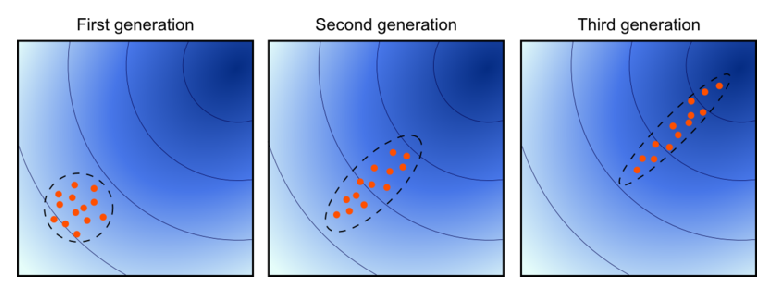
\includegraphics[height=0.35\columnwidth]{CMA-ES}
\end{figure}
}


\frame{\frametitle{Size of training set}
\bi Small sample of training individuals of known fitness are needed to generate an initial surrogate. 
\item Size of training set is denoted $\overline{\ell}$. Note if training size is unlimited then updating the surrogate becomes computationally expensive, and therefore needs to be pruned.
\ei 
}
\frame{\vspace{-0.2cm}\frametitle{Anova plot for different validation strategies:}
\begin{figure}[b!]
\centering
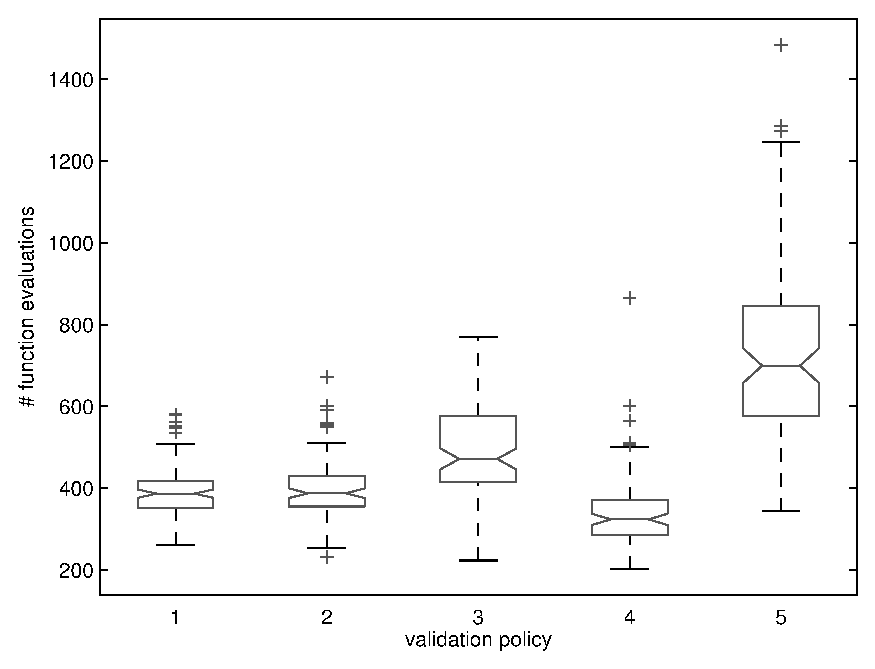
\includegraphics[height=0.45\columnwidth]{anova}
\caption{1) prune old individuals, 2) prune bad individuals, 3) adding a pseudo mean candidate individual 4) correctly rank $\mu$ best ranked candidate individuals 5) update on every other generation for Rosenbrock's function for dimension $n=2$}
\end{figure}
}
\frame{\frametitle{Completely concordant ranking}
\bi If the training accuracy is not 100\% then  $\tau<1$
\bi resulting in additional training individuals to be forced for evaluation. \ei
\item However, since the search is stochastic this is deemed to strict, thus a sufficiently accurate surrogate would be if $\tau>0.999$. 
\ei
}
\frame{\frametitle{Schema for the sampling strategy}
{\centering \begin{figure}[t!]
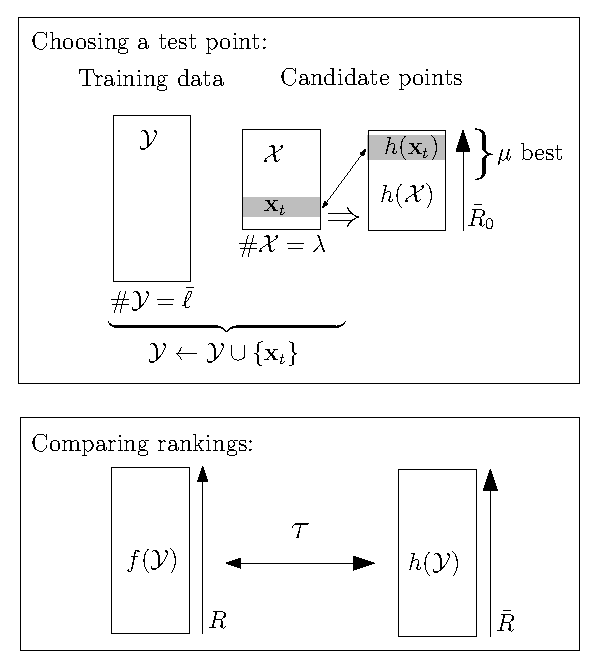
\includegraphics[width=0.5\columnwidth]{schema}
\end{figure}}
}
\section{Experimental Study}
\subsection{Sphere model and Rosenbrock's function}
\frame{\frametitle{Classical Optimisation Problems}
\bi Sphere model, for dimension $n=2,5,10,20$:
$$f(\vec{x})=\sum_{k=1}^n x_k^2$$
\item Rosenbrock's function, for dimension $n=2,5,10,20$:
$$f(\vec{x})=\sum_{k=2}^n 100(x_k-x_{k-1}^2)^2+(1-x_{k-1})^2$$
\ei
}
\frame{\frametitle{Main statistics of experimental results for sphere model.}
\begin{table}[t!] 
\centering
{\renewcommand{\arraystretch}{1.1} %\renewcommand{\tabcolsep}{0.02cm} 
\footnotesize
%\begin{tabularx}{0.99\columnwidth}{| X | c | rrr | rrr| }%rrr |}
\begin{tabular}{| l | c | rrr | rrr| }%rrr |}
\hline
 & & \multicolumn{3}{c|}{Function eval.} & \multicolumn{3}{c|}{Generations} \\%& \multicolumn{3}{c|}{Fitness} \\ 
     & $n$ & \multicolumn{1}{c}{mean} & \multicolumn{1}{c}{median} & \multicolumn{1}{c|}{sd} & \multicolumn{1}{c}{mean} & \multicolumn{1}{c}{median} & \multicolumn{1}{c|}{sd} \\%& \multicolumn{1}{|c}{mean} & \multicolumn{1}{c}{median} & \multicolumn{1}{c|}{sd} \\
\hline
all& 2 & 130.59 & 132 & 18.33 & 49.02 & 49 & 6.51 \\%& 2.35e-09 & 2.82e-10 & 1.15e-08\\ 
$\mu$&2 &{\bf 81.53}& 81 & 9.53 &{\bf 48.11 }& 48 & 5.02 \\%& 7.01e-10 & 2.26e-10 & 1.35e-09\\ 
\hline
all& 5 & 702.02 & 702 & 67.57 & 145.15 & 145 & 14.96 \\%& 2.77e-10 & 1.82e-10 & 3.64e-10\\ 
$\mu$& 5 & {\bf 545.25}& 547 & 54.27 & {\bf 132.60}& 132 & 11.03 \\%& 1.83e-10 & 1.46e-10 & 1.09e-10\\ 
\hline
all& 10 & 1563.58 & 1553 & 117.09 & 241.83 & 240 & 18.47 \\%& 1.52e-10 & 1.37e-10 & 5.03e-11\\ 
$\mu$& 10 & {\bf 1161.03 }& 1158 & 79.98 & {\bf 226.60} & 224 & 13.86\\% & 1.34e-10 & 1.22e-10 & 3.80e-11\\ 
\hline
all& 20 & 3383.83 & 3377 & 135.52 & 423.14 & 424 & 20.42 \\%& 1.27e-10 & 1.21e-10 & 2.51e-11\\ 
$\mu$& 20 & {\bf 2795.28} & 2804 & 132.77 & {\bf 372.86} & 372 & 16.56 \\%& 1.17e-10 & 1.12e-10 & 1.72e-11\\ 
\hline
\end{tabular}
}
\end{table}
}

\frame{\frametitle{Main statistics of experimental results for Rosenbrock's function.}
\begin{table}[t!]
\centering
{\renewcommand{\arraystretch}{1.1} %\renewcommand{\tabcolsep}{0.02cm} 
\footnotesize
%\begin{tabularx}{0.99\columnwidth}{| X | c | rrr | rrr| }%rrr |}
\begin{tabular}{| l | c | rrr | rrr| }%rrr |}
\hline
 & & \multicolumn{3}{c|}{Function eval.} & \multicolumn{3}{c|}{Generations} \\%& \multicolumn{3}{c|}{Fitness} \\ 
     & $n$ & \multicolumn{1}{c}{mean} & \multicolumn{1}{c}{median} & \multicolumn{1}{c|}{sd} & \multicolumn{1}{c}{mean} & \multicolumn{1}{c}{median} & \multicolumn{1}{c|}{sd} \\%& \multicolumn{1}{|c}{mean} & \multicolumn{1}{c}{median} & \multicolumn{1}{c|}{sd} \\
\hline
all & 2 & 389.85 & 386 & 63.85 & {\bf 132.31} & 130 & 31.25 \\%& 6.24e-10 & 3.20e-10 & 1.05e-09\\ 
$\mu$ & 2 &{\bf 344.91} & 336 & 78.58 & 172.16 & 170 & 49.95 \\%& 7.53e-10 & 1.66e-10 & 3.64e-09\\ 
\hline
all & 5 & 2464.22 & 2280 & 748.55 & {\bf 514.59} & 492 & 105.77 \\%& 2.75e-01 & 1.74e-10 & 1.01e+00\\ 
$\mu$ & 5 & {\bf 1724.89} & 1729 & 295.60 & 520.66 & 520 & 82.79 \\%& 1.83e-10 & 1.53e-10 & 1.05e-10\\ 
\hline
all & 10 & 6800.50 & 6495 & 1258.68 & {\bf 1079.82} & 1052 & 177.76 \\%& 2.79e-01 & 1.32e-10 & 1.02e+00\\ 
$\mu$ & 10 & {\bf 6138.48} & 6143 & 1398.15 & 1177.71 & 1103 & 310.11 \\%& 1.99e-01 & 1.24e-10 & 8.73e-01\\ 
\hline
all & 20 & 19968.80 & 20004 & 234.66 &{\bf 2494.00} & 2500 & 49.60 \\%& 4.54e-01 & 2.88e-02 & 1.08e+00\\ 
$\mu$ & 20 &{\bf 19645.90 }& 20002 & 1086.37 & 2687.25 & 2748 & 230.50 \\%& 3.10e-01 & 3.12e-07 & 9.97e-01\\ 
\hline
\end{tabular}
}
\end{table}
}


\section{Main Conclusions and Future Work}\subsection{Main Conclusions and Future Work}
{\frame{\frametitle{Main Conclusions}
\bi The new validation approach reduces the number of fitness evaluations, without a loss in performance although it might take a few more iterations in CMA-ES.
	\item Sampling used for validation of the accuracy of the surrogate can stop once the $\mu$ best ranked candidate individuals have been evaluated 
	\bi since they are the only candidate individuals who will survive to become parents in the next generation \ei
	\item In some cases the sampling could have stopped sooner, when the surrogate ranking was sufficiently concordant.%, i.e. $\tau$ was close enough to 1
	\item No statistical difference between omitting oldest or lowest ranking individuals from training set.
\ei
}

{\frame{\frametitle{Future Work}
\bi Further investigation on the fitness landscape to determine more effectively points of interest (and no longer of interest).
	\bi e.g. disregarding points with the greatest euclidean distance from the current candidate individuals \ei
	\item  The allowable range for $\tau\in[0.999,1]$ might be too narrow an interval, resulting in an excess of expensive function evaluations needed.
	\item This is a simple case study, and the framework needs to be implemented on a greater range of test functions, e.g. job shop scheduling problem. 
\ei
}


\end{document}
%%%%%%%%%%%%%%%%%%%%%%%%%%%%%%%%%%%%%%%
